\ifx\allfiles\undefined
\documentclass[12pt, a4paper, oneside, UTF8]{ctexbook}
\def\path{../../config}
\usepackage{amsmath}
\usepackage{amsthm}
\usepackage{amssymb}
\usepackage{array}
\usepackage{xcolor}
\usepackage{graphicx}
\usepackage{mathrsfs}
\usepackage{enumitem}
\usepackage{geometry}
\usepackage[colorlinks, linkcolor=black]{hyperref}
\usepackage{stackengine}
\usepackage{yhmath}
\usepackage{extarrows}
\usepackage{tikz}
\usepackage{pgfplots}
\usepackage{asymptote}
\usepackage{float}
\usepackage{fontspec} % 使用字体

\setmainfont{Times New Roman}
\setCJKmainfont{LXGWWenKai-Light}[
    SlantedFont=*
]

\everymath{\displaystyle}

\usepgfplotslibrary{polar}
\usepackage{subcaption}
\usetikzlibrary{decorations.pathreplacing, positioning}

\usepgfplotslibrary{fillbetween}
\pgfplotsset{compat=1.18}
% \usepackage{unicode-math}
\usepackage{esint}
\usepackage[most]{tcolorbox}

\usepackage{fancyhdr}
\usepackage[dvipsnames, svgnames]{xcolor}
\usepackage{listings}

\definecolor{mygreen}{rgb}{0,0.6,0}
\definecolor{mygray}{rgb}{0.5,0.5,0.5}
\definecolor{mymauve}{rgb}{0.58,0,0.82}
\definecolor{NavyBlue}{RGB}{0,0,128}
\definecolor{Rhodamine}{RGB}{255,0,255}
\definecolor{PineGreen}{RGB}{0,128,0}

\graphicspath{ {figures/},{../figures/}, {config/}, {../config/} }

\linespread{1.6}

\geometry{
    top=25.4mm, 
    bottom=25.4mm, 
    left=20mm, 
    right=20mm, 
    headheight=2.17cm, 
    headsep=4mm, 
    footskip=12mm
}

\setenumerate[1]{itemsep=5pt,partopsep=0pt,parsep=\parskip,topsep=5pt}
\setitemize[1]{itemsep=5pt,partopsep=0pt,parsep=\parskip,topsep=5pt}
\setdescription{itemsep=5pt,partopsep=0pt,parsep=\parskip,topsep=5pt}

\lstset{
    language=Mathematica,
    basicstyle=\tt,
    breaklines=true,
    keywordstyle=\bfseries\color{NavyBlue}, 
    emphstyle=\bfseries\color{Rhodamine},
    commentstyle=\itshape\color{black!50!white}, 
    stringstyle=\bfseries\color{PineGreen!90!black},
    columns=flexible,
    numbers=left,
    numberstyle=\footnotesize,
    frame=tb,
    breakatwhitespace=false,
} 

\lstset{
    language=TeX, % 设置语言为 TeX
    basicstyle=\ttfamily, % 使用等宽字体
    breaklines=true, % 自动换行
    keywordstyle=\bfseries\color{NavyBlue}, % 关键字样式
    emphstyle=\bfseries\color{Rhodamine}, % 强调样式
    commentstyle=\itshape\color{black!50!white}, % 注释样式
    stringstyle=\bfseries\color{PineGreen!90!black}, % 字符串样式
    columns=flexible, % 列的灵活性
    numbers=left, % 行号在左侧
    numberstyle=\footnotesize, % 行号字体大小
    frame=tb, % 顶部和底部边框
    breakatwhitespace=false % 不在空白处断行
}

% \begin{lstlisting}[language=TeX] ... \end{lstlisting}

% 定理环境设置
\usepackage[strict]{changepage} 
\usepackage{framed}

\definecolor{greenshade}{rgb}{0.90,1,0.92}
\definecolor{redshade}{rgb}{1.00,0.88,0.88}
\definecolor{brownshade}{rgb}{0.99,0.95,0.9}
\definecolor{lilacshade}{rgb}{0.95,0.93,0.98}
\definecolor{orangeshade}{rgb}{1.00,0.88,0.82}
\definecolor{lightblueshade}{rgb}{0.8,0.92,1}
\definecolor{purple}{rgb}{0.81,0.85,1}

\theoremstyle{definition}
\newtheorem{myDefn}{\indent Definition}[section]
\newtheorem{myLemma}{\indent Lemma}[section]
\newtheorem{myThm}[myLemma]{\indent Theorem}
\newtheorem{myCorollary}[myLemma]{\indent Corollary}
\newtheorem{myCriterion}[myLemma]{\indent Criterion}
\newtheorem*{myRemark}{\indent Remark}
\newtheorem{myProposition}{\indent Proposition}[section]

\newenvironment{formal}[2][]{%
	\def\FrameCommand{%
		\hspace{1pt}%
		{\color{#1}\vrule width 2pt}%
		{\color{#2}\vrule width 4pt}%
		\colorbox{#2}%
	}%
	\MakeFramed{\advance\hsize-\width\FrameRestore}%
	\noindent\hspace{-4.55pt}%
	\begin{adjustwidth}{}{7pt}\vspace{2pt}\vspace{2pt}}{%
		\vspace{2pt}\end{adjustwidth}\endMakeFramed%
}

\newenvironment{definition}{\vspace{-\baselineskip * 2 / 3}%
	\begin{formal}[Green]{greenshade}\vspace{-\baselineskip * 4 / 5}\begin{myDefn}}
	{\end{myDefn}\end{formal}\vspace{-\baselineskip * 2 / 3}}

\newenvironment{theorem}{\vspace{-\baselineskip * 2 / 3}%
	\begin{formal}[LightSkyBlue]{lightblueshade}\vspace{-\baselineskip * 4 / 5}\begin{myThm}}%
	{\end{myThm}\end{formal}\vspace{-\baselineskip * 2 / 3}}

\newenvironment{lemma}{\vspace{-\baselineskip * 2 / 3}%
	\begin{formal}[Plum]{lilacshade}\vspace{-\baselineskip * 4 / 5}\begin{myLemma}}%
	{\end{myLemma}\end{formal}\vspace{-\baselineskip * 2 / 3}}

\newenvironment{corollary}{\vspace{-\baselineskip * 2 / 3}%
	\begin{formal}[BurlyWood]{brownshade}\vspace{-\baselineskip * 4 / 5}\begin{myCorollary}}%
	{\end{myCorollary}\end{formal}\vspace{-\baselineskip * 2 / 3}}

\newenvironment{criterion}{\vspace{-\baselineskip * 2 / 3}%
	\begin{formal}[DarkOrange]{orangeshade}\vspace{-\baselineskip * 4 / 5}\begin{myCriterion}}%
	{\end{myCriterion}\end{formal}\vspace{-\baselineskip * 2 / 3}}
	

\newenvironment{remark}{\vspace{-\baselineskip * 2 / 3}%
	\begin{formal}[LightCoral]{redshade}\vspace{-\baselineskip * 4 / 5}\begin{myRemark}}%
	{\end{myRemark}\end{formal}\vspace{-\baselineskip * 2 / 3}}

\newenvironment{proposition}{\vspace{-\baselineskip * 2 / 3}%
	\begin{formal}[RoyalPurple]{purple}\vspace{-\baselineskip * 4 / 5}\begin{myProposition}}%
	{\end{myProposition}\end{formal}\vspace{-\baselineskip * 2 / 3}}


\newtheorem{example}{\indent \color{SeaGreen}{Example}}[section]
\renewcommand{\proofname}{\indent\textbf{\textcolor{TealBlue}{Proof}}}
\NewEnviron{solution}{%
	\begin{proof}[\indent\textbf{\textcolor{TealBlue}{Solution}}]%
		\color{blue}% 设置内容为蓝色
		\BODY% 插入环境内容
		\color{black}% 恢复默认颜色(可选,避免影响后续文字)
	\end{proof}%
}

% 自定义命令的文件

\def\d{\mathrm{d}}
\def\R{\mathbb{R}}
%\newcommand{\bs}[1]{\boldsymbol{#1}}
%\newcommand{\ora}[1]{\overrightarrow{#1}}
\newcommand{\myspace}[1]{\par\vspace{#1\baselineskip}}
\newcommand{\xrowht}[2][0]{\addstackgap[.5\dimexpr#2\relax]{\vphantom{#1}}}
\newenvironment{mycases}[1][1]{\linespread{#1} \selectfont \begin{cases}}{\end{cases}}
\newenvironment{myvmatrix}[1][1]{\linespread{#1} \selectfont \begin{vmatrix}}{\end{vmatrix}}
\newcommand{\tabincell}[2]{\begin{tabular}{@{}#1@{}}#2\end{tabular}}
\newcommand{\pll}{\kern 0.56em/\kern -0.8em /\kern 0.56em}
\newcommand{\dive}[1][F]{\mathrm{div}\;\boldsymbol{#1}}
\newcommand{\rotn}[1][A]{\mathrm{rot}\;\boldsymbol{#1}}

\newif\ifshowanswers
\showanswerstrue % 注释掉这行就不显示答案

% 定义答案环境
\newcommand{\answer}[1]{%
    \ifshowanswers
        #1%
    \fi
}

% 修改参数改变封面样式,0 默认原始封面、内置其他1、2、3种封面样式
\def\myIndex{0}


\ifnum\myIndex>0
    \input{\path/cover_package_\myIndex} 
\fi

\def\myTitle{考研数学笔记}
\def\myAuthor{Weary Bird}
\def\myDateCover{\today}
\def\myDateForeword{\today}
\def\myForeword{相见欢·林花谢了春红}
\def\myForewordText{
    林花谢了春红,太匆匆。
    无奈朝来寒雨晚来风。
    胭脂泪,相留醉,几时重。
    自是人生长恨水长东。
}
\def\mySubheading{以姜晓千强化课讲义为底本}




\begin{document}
\input{\path/cover_text_\myIndex.tex}

\newpage
\thispagestyle{empty}
\begin{center}
    \Huge\textbf{\myForeword}
\end{center}
\myForewordText
\begin{flushright}
    \begin{tabular}{c}
        \myDateForeword
    \end{tabular}
\end{flushright}

\newpage
\pagestyle{plain}
\setcounter{page}{1}
\pagenumbering{Roman}
\tableofcontents

\newpage
\pagenumbering{arabic}
% \setcounter{chapter}{-1}
\setcounter{page}{1}

\pagestyle{fancy}
\fancyfoot[C]{\thepage}
\renewcommand{\headrulewidth}{0.4pt}
\renewcommand{\footrulewidth}{0pt}








\else
\fi

\chapter{多元函数微分学}
\section{多元函数的概念}

\begin{remark}
    多元函数微分学的概念 \\
    \underline{可微的概念} 设二元函数$f(x,y)$在点$(x_0,y_0)$的某领域内有定义,且其全增量可以写成
    $$
    \Delta z = f(x_0+\Delta x, y_0+\Delta y) - f(x_0,y_0) = A\Delta x + B\Delta y + o(\rho)
    $$
    其中$\rho=\sqrt{(\Delta x)^2+(\Delta y)^2}$
    其中$A,B$为不依赖于$\Delta x,\Delta y$,而仅与$x_0,y_0$有关,则其在$(x_0,y_0)$可微 \\
    \underline{全微分} 若$f(x,y)$在$(x_0,y_0)$可微,则其全微分为
    $$
    \d z = A\Delta x + B\Delta y \xlongequal{\text{可微的必要条件}} f'_{x}(x_0,y_0)\d x + f'_{y}(x_0,y_0)\d y
    $$
    \underline{可微的必要条件} 若$f(x,y)$在点$(x_0,y_0)$可微,则$f(x,y)$在该点连续,且两个偏导数都存在 \\
    \underline{可微的充分条件} 若$f(x,y)$在点$(x_0,y_0)$处偏导数存在,且作为二元函数在该点连续,则$f(x,y)$在点$(x_0,y_0)$可微
\end{remark}
\begin{enumerate}[label=\arabic*.]
    \item 例1 求下列重极限: \\
        (1)$\displaystyle \lim_{\substack{x\to 0\\ y\to 0}}\frac{x^\alpha y^\beta}{x^2+y^2}\quad (\alpha\geq0,\beta\geq0)$; \\
        (2)$\displaystyle \lim_{\substack{x\to 0\\ y\to 0}}\frac{xy(x^{2}-y^{2})}{x^{2}+y^{2}}$; \\
        (3)$\displaystyle \lim_{\substack{x\to 0\\ y\to 0}}\frac{x^2y^2}{(x^2+y^2)^{\frac{3}{2}}}$
    
    \begin{solution}
    (1)即总结 \\
    (2)重极限也满足极限的四则运算故
    $$
    \text{原式}=\lim_{\substack{x\to 0\\y\to 0}}\frac{x^3y}{x^2+y^2}-\lim_{\substack{x\to 0\\y\to 0}}\frac{xy^3}{x^2+y^2} 
    $$
    由结论可知$\text{原式}=0$ \\
    (3)
    $$
    \text{原式}=\lim_{\substack{x\to 0\\y\to 0}}\left(\frac{x^{\frac{4}{3}}y^{\frac{4}{3}}}{x^2+y^2}\right)^{\frac{3}{2}} = 0
    $$
    \end{solution}
    
    \begin{tcolorbox}[title=求重极限的技巧]
    若需要计算重极限,考虑极坐标换元通常比较简单.对于形如
    $$
    \lim_{\substack{x\to 0\\ y\to 0}}\frac{x^{\alpha}y^{\beta}}{x^2+y^2} 
    $$
    只需要做极坐标换元即可
    \begin{align*}
        \text{原式} &= \lim_{r\to 0^{+}}
        \frac{r^{\alpha+\beta}\cos^{\alpha}{\theta}\sin^{\beta}{\theta}}{r^2},(\theta\in\left[0,2\pi\right]) \\
        &=\begin{cases}
            0, &\alpha + \beta - 2 > 0 \\
            \text{不存在}, &\alpha + \beta - 2 \leq 0
        \end{cases}
    \end{align*}
    \end{tcolorbox}

    \item (2012,数一)如果函数$f(x,y)$在点$(0,0)$处连续,那么下列命题正确的是 \\
    $\displaystyle (A)\ \text{若极限}\lim_{\substack{x\to 0\\ y\to 0}}\frac{f(x,y)}{|x|+|y|}\text{存在,则}f(x,y)\text{在点}(0,0)\text{处可微}$ \\
    $\displaystyle (B)\ \text{若极限}\lim_{\substack{x\to 0\\ y\to 0}}\frac{f(x,y)}{x^{2}+y^{2}}\text{存在,则}f(x,y)\text{在点}(0,0)\text{处可微}$ \\
    $\displaystyle (C)\ \text{若}f(x,y)\text{在点}(0,0)\text{处可微,则极限}\lim_{\substack{x\to 0\\ y\to 0}}\frac{f(x,y)}{|x|+|y|}\text{存在}$ \\
    $\displaystyle (D)\ \text{若}f(x,y)\text{在点}(0,0)\text{处可微,则极限}\lim_{\substack{x\to 0\\ y\to 0}}\frac{f(x,y)}{x^{2}+y^{2}}\text{存在}$

    \begin{solution}
    (方法一)证明B选项正确
    $$
    \lim_{\substack{x\to 0\\y\to 0}}\frac{f(x,y)}{x^2+y^2}\exists,\text{且}f(x,y)\text{连续}\implies f(0,0) = 0 
    $$
    {\color{red} 脱极限号}有
    $$
        f(x,y) = o(\rho) 
    $$
    由可微的定义有
    $$
        f(x,y)-f(0,0)=0\cdot\Delta x + 0\cdot\Delta y + o(\rho)
    $$
    从而$f(x,y)$在$(0,0)$可微 \\
    (方法二)特殊值证明$ACD$不正确 \\
    对于A选项,当$f(x)=\left|x\right|+\left|y\right|$ 不可微 \\
    对于CD选项,当$f(x,y)=C\neq 0$的时候,极限不存在
    \end{solution}

    \item (2012,数三)设连续函数$z=f(x,y)$满足
    \begin{align*}
        \lim_{\substack{x\to 0\\ y\to 1}}\frac{f(x,y)-2x+y-2}{\sqrt{x^2+(y-1)^2}}=0
    \end{align*}
    则$\left.dz\right|_{(0,1)}=$
    
    \begin{solution}
    (方法一)和上面的题目比较相似,由题设可知$f(0,1)=1$,脱极限号有
    $$
    f(x,y)-2x+y-2=o(\rho)
    $$
    由可微的定义有
    $$
    f(x,y)-1=2x-(y-1)+o(\rho) = 2\Delta x - \Delta + o(\rho)
    $$
    即
    $$
    d\big|_{(0,1)}=2\d x-\d y
    $$
    (方法二)特殊值 令$f(x,y)=2x-y+2$,可以直接求出$d\big|_{(0,1)}=2\d x-\d y$
    \end{solution}
\end{enumerate}

\section{多元复合函数求偏导数与全微分}

\begin{remark}
    本质是计算题,仔细计算即可. 注意点 \\
    (一) 链式法则 \\
    (二) 一阶全微分形式不变性 \\
    (三) 二阶混合偏导数若连续则相等 
\end{remark}

\begin{enumerate}[label=\arabic*.,start=4]
    \item (2021,数一、数二、数三)设函数$f(x,y)$可微,且$f(x+1,e^x)=x(x+1)^2,f(x,x^2)=2x^2\ln x$
    则$df(1,1)=$ \\
    $(A)\ dx+dy \quad (B)\ dx-dy \quad (C)\ dy\qquad (D)\ \d y$
    
    \begin{solution}
    第一个等式两边同时对$x$求导有
    $$
    f'_1(x+1,e^x)+f'_2(x+1,e^x)e^x=(x+1)^2+2x(x+1)
    $$
    令$x=0$则
    $$
    f'_1(1,1)+f'_2(1,1)=1
    $$
    同理,第二个等式两边同时对$x$求导有
    $$
    f'_1(x,x^2)+f'_2(x,x^2)\cdot 2x = 4x\ln{x}+2x 
    $$
    令$x=1$则
    $$
    f'_1(1,1)+2f'_2(1,1)=2
    $$
    联立可以解出
    $$
    \begin{cases}
        f'_1{(1,1)}=0 \\
        f'_2{(1,1)}=1
    \end{cases}
    $$
    故$\d f(1,1)=\d y$
    \end{solution}
    
    \item (2011,数一、数二)设$z=f(xy,yg(x))$,其中函数$f$具有二阶连续偏导数,函数$g(x)$可导,且在$x=1$处取得极值$g(1)=1$,
    求$\displaystyle\left.\frac{\partial^2 z}{\partial x\partial y}\right|_{x=1,y=1}$。
    
    \begin{solution}
    由题设可知$g'(1)=0,g(1)=0$ 且
    $$
    \frac{\partial z}{\partial x} = f'_1\cdot y + f'_1\cdot y g'(x) 
    $$
    {\color{red}这种求值的题目先带入可以化简} 
    $$
    \frac{\partial z}{\partial x}\big|_{(x=1)} = f'_1\cdot y 
    $$
    $$
    \frac{\partial^2 z}{\partial x\partial y}\big|_{(x=1)} = f''_{11}\cdot y + f'_1 + f''_{12}\cdot g(x) 
    $$
    带入$y=1$有
    $$
    \frac{\partial^2 z}{\partial x\partial y}\big|_{(x=1,y=1)} = f''_{11}(1,1)+f'_{1}(1,1)+f''_{12}(1,1)
    $$
    \end{solution}
\end{enumerate}

\section{多元隐函数求偏导数与全微分}
\begin{remark}
    三个方法 \\
    (方法一)代入求偏导$z=z(x,y)$ \\
    {\color{red} (方法二)公式法} $\displaystyle \frac{\partial z}{\partial x} =-\frac{F'_x}{F'_z}$; 
    $\displaystyle \frac{\partial z}{\partial y} =-\frac{F'_y}{F'_z}$ \\
    (方法三)全微分
\end{remark}
\begin{enumerate}[label=\arabic*.,start=6]
    \item (2005,数一)设有三元方程$xy-z\ln y+e^{xz}=1$,根据隐函数存在定理,存在点$(0,1,1)$的一个邻域,在此邻域内该方程 \\
    (A)\ \text{只能确定一个具有连续偏导数的隐函数}$z=z(x,y)$ \\
    (B)\ \text{可确定两个具有连续偏导数的隐函数}$x=x(y,z)$\text{和}$z=z(x,y)$ \\
    (C)\ \text{可确定两个具有连续偏导数的隐函数}$y=y(x,z)$\text{和}$z=z(x,y)$ \\
    (D)\ \text{可确定两个具有连续偏导数的隐函数}$x=x(y,z)$\text{和}$y=y(x,z)$

    \begin{solution}
    由题设有$F(x,y,z)=xy-2\ln{y}+e^{xz}-1$ 分别对$x,y,z$求导有
    $$
    \begin{cases}
        F'_x(0,1,1)=2\neq 0 \\
        F'_y(0,1,1)=-2\neq 0 \\
        F'_z(0,1,1)=0 
    \end{cases}
    $$
    由隐函数存在定理可知仅$x,y$可以作为因变量
    \end{solution}
    
    \begin{tcolorbox}[title=隐函数存在定理]
        (隐函数存在定理)如果二元函数$F(x,y)=0$,满足如下三个条件
        \begin{enumerate}
            \item [(1)] 函数$F(x,y)$在点$(x_0,y_0)$某邻域内有连续偏导数
            \item [(2)] $F(x_0,y_0)=0$ 
            \item [(3)] $F;(x_0,y_0)\neq 0$
        \end{enumerate}
        则方程$F(x,y)=0$在点$(x_0,y_0)$某邻域内恒能{\color{red}唯一}确定一个连续函数$y=y(x)$,且
        $$
        y' = \frac{\d y}{\d x} = -\frac{F'_x}{F'_y}
        $$
        {\color{red} 简单来说对谁的偏导数不为零,谁能表示为其余变量的函数(作为因变量)}
    \end{tcolorbox}
    \item (1999,数一)设$y=y(x),z=z(x)$是由方程$z=xf(x+y)$和$F(x,y,z)=0$所确定的函数,其中$f$和$F$分别具有一阶连续导数和一阶连续偏导数,求$\frac{dz}{dx}$。
    
    \begin{solution}
    记
    \begin{align}
        z=xf(x+y) \tag{1} \\
        F(x,y,z)=0 \tag{2}
    \end{align}
    分别对(1)和(2)的两端对x/y求导有 
    \begin{align*}
        \frac{\d z}{\d x} = f(x+y) + xf'(1+\frac{\d y}{\d x}) \tag{3} \\
        F'_1 + F'_2\frac{\d y}{\d x} + F'_3\frac{\d z}{\d x} = 0 \tag{4}
    \end{align*}
    联立(3)和(4)可以解出 
    $$
    \frac{\d z}{\d x} = \frac{(f+xf')F'_2-xf'F'_1}{F'_2+xf'\cdot F'_3}
    $$
    \end{solution}

    \begin{tcolorbox}[title=多元函数组确认函数的情况]
        本质是方程组思想 \\
        {\color{red}一个三元方程可以确定一个二元函数} \\
        {\color{red}二个三元方程可以确定两个二元函数} \\
        参考线性代数的方程组的解,就很容易明白
    \end{tcolorbox}
\end{enumerate}

\section{变量代换化简偏微分方程}

\begin{enumerate}[label=\arabic*.,start=8]
    \item (2010,数二)设函数$u=f(x,y)$具有二阶连续偏导数,且满足等式
    \begin{align*}
        4\frac{\partial^2 u}{\partial x^2}+12\frac{\partial^2 u}{\partial x\partial y}+5\frac{\partial^2 u}{\partial y^2}=0
    \end{align*}
    确定$a,b$的值,使等式在变换$\xi=x+ay,\eta=x+by$下简化为$\frac{\partial^2 u}{\partial \xi\partial \eta}=0$。
    
    \begin{solution}
    有题设有 
    $$
    \begin{cases}
        \displaystyle 
        \frac{\partial u}{\partial x} = \frac{\partial u}{\partial \xi} + \frac{\partial u}{\partial \eta} \\
        \displaystyle
        \frac{\partial^2 u}{\partial x^2} = \frac{\partial^2 u}{\partial \xi^2} + 2\frac{\partial^2 u}{\partial\xi\partial\eta}
        +\frac{\partial^2 u}{\partial \eta^2} \\
        \displaystyle
        \frac{\partial^2 u}{\partial y^2} = a^2\frac{\partial^2 u}{\partial \xi^2} + 2ab\frac{\partial^2 u}{\partial\xi\partial\eta}
        +b^2\frac{\partial^2 u}{\partial \eta^2} \\
        \displaystyle 
        \frac{\partial^2 u}{\partial x\partial y} = a\frac{\partial^2 u}{\partial \xi^2} + (a+b)\frac{\partial^2 u}{\partial\xi\partial\eta}
        +b\frac{\partial^2 u}{\partial \eta^2} 
    \end{cases}
    $$
    带入题设等式有
    $$
    \begin{cases}
        a = 2 \\
        b = -\frac{2}{5}
    \end{cases} \text{或} 
    \begin{cases}
        a = -\frac{2}{5} \\
        b = -2
    \end{cases}
    $$
    \end{solution}
\end{enumerate}
\section{求无条件极值}
\begin{remark}
    两个方法 \\
    (一)多元函数微分学的定义
    $$
    \begin{cases}
        \text{是极值,一般使用保号性证明} \\
        \text{不是极值,一般取不同路径}
    \end{cases}
    $$
    (二)$AC-B^2$判别法,若$\color{red} f'_x=f'_y=0$且其二阶偏导数存在,记
    $$
    \begin{cases}
        A=f''_{xx} \\
        B=f''_{xy} \\
        C=f''_{yy} 
    \end{cases} \implies AC-B^2\begin{cases}
        > 0, &\begin{cases}
            A > 0, &\text{极小值} \\
            A < 0, &\text{极大值}
        \end{cases} \\
        < 0, &\text{不是} \\
        = 0, &\text{判别法失效,无法判断}
    \end{cases}
    $$
\end{remark}
\begin{enumerate}[label=\arabic*.,start=9]
    \item (2003,数一)已知函数$f(x,y)$在点$(0,0)$的某个邻域内连续,且
    \begin{align*}
        \lim_{\substack{x\to 0\\ y\to 0}}\frac{f(x,y)-xy}{(x^2+y^2)^2}=1
    \end{align*}
    则 \\
    $(A)\ \text{点}(0,0)\text{不是}f(x,y)\text{的极值点}$ \\
    $(B)\ \text{点}(0,0)\text{是}f(x,y)\text{的极大值点}$ \\
    $(C)\ \text{点}(0,0)\text{是}f(x,y)\text{的极小值点}$ \\
    $(D)\ \text{根据所给条件无法判别点}(0,0)\text{是否为}f(x,y)\text{的极值点}$
    
    \begin{solution}
    有题设可知$f(0,0)=0$ \\
    方法一: 选特殊路径证明,脱极限号有 $\displaystyle f(x,y)=xy+o(x^2+y^2)$ \\
    令$y=x,f(x,x)=x^2+o(x^2) > 0$ \\
    令$y=-x,f(x,-x)=-x^2+O(x^2) < 0$ \\
    故点$(0,0)$不是$f(x,y)$的极值点 \\
    方法二: 特殊值用判别法证明, 不妨假设$f(xy)=xy+(x^2+y^2)^2$ 且$\displaystyle \frac{\partial f}{\partial x}\big|_{(0,0)}
    =\frac{\partial f}{\partial y}\big|_{(0,0)}=0$
    而$A=0,B=1,C=0 \implies AC-B^2=-1<0$ 故$(0,0)$不是极值 
    \end{solution}
    
    \item (2004,数一)设$z=z(x,y)$是由$x^2-6xy+10y^2-2yz-z^2+18=0$确定的函数,求$z=z(x,y)$的极值点和极值。
    
    \begin{solution}
    对于这种题分两步,第一步求驻点,第二步求二阶偏导数并用判别法判断所有驻点.题目等式两边分别对{x,y}求导有 
    \begin{align}
        & \text{对}x\text{求导} 2x-6y-2y\frac{\partial z}{\partial x} - 2z\frac{\partial z}{\partial x} = 0 \tag{1} \label{eq1} \\
        & \text{对}y\text{求导} -6x + 20y - 2z - 2y\frac{\partial z}{\partial y} - 2z\frac{\partial z}{\partial y} = 0 \tag{2} \label{eq2}
    \end{align}
    令$\displaystyle \frac{\partial z}{\partial y}=\frac{\partial z}{\partial x}=0$ 有$\begin{cases}
        x = 3y \\
        y = z
    \end{cases}$ 带入题设等式有可以解出
    $$
    \begin{cases}
        x = 9 \\
        y = z = 3 
    \end{cases} \text{或}
    \begin{cases}
        x = -9 \\
        y = z = -3
    \end{cases}
    $$
    对\eqref{eq1}两侧对$x,y$求导有,且带入$\displaystyle \frac{\partial z}{\partial y}=\frac{\partial z}{\partial x}=0$
    \begin{align}
        & 2 - 2y\frac{\partial^2 z}{\partial x^2} - 2z\frac{\partial^2 z}{\partial x^2} = 0 \tag{3} \\
        & -6 - 2y\frac{\partial^2 z}{\partial x\partial y} - 2z\frac{\partial^2 z}{\partial x\partial y} = 0 \tag{4}
    \end{align}
    对\eqref{eq2}两测对$y$求导有,且带入$\displaystyle \frac{\partial z}{\partial y}=\frac{\partial z}{\partial x}=0$
    \begin{align}
        20 - 2y\frac{\partial^2 z}{\partial y^2}-2z\frac{\partial^2 z}{\partial x\partial y} = 0 \tag{5}
    \end{align}
    综上可以解出
    $$
    \begin{cases}
        \displaystyle \frac{\partial^2 z}{\partial x^2} = \frac{1}{y+z} \\
        \displaystyle \frac{\partial^2 z}{\partial x\partial y} = \frac{-3}{y+z} \\
        \displaystyle \frac{\partial^2 z}{\partial y^2} = \frac{10}{y+z}
    \end{cases}
    $$
    带入题设条件可知
    $$
    \begin{cases}
        \text{对于点}(9,3,3) AC-B^2 > 0,\text{且} A > 0,\text{故}z(9,3)\text{为极小值} \\
        \text{对于点}(-9,-3,-3) AC-B^2 > 0,\text{且} A < 0,\text{故}z(-9,-3)\text{为极大值}
    \end{cases}
    $$
    \end{solution}
\end{enumerate}

\section{求条件极值(边界最值)}
\begin{remark}
    (方法一)lagrange乘数法 \\
    构造辅助函数$L(x,y,\lambda)=f(x,y)+\lambda\cdot\varphi(x,y)$ 然后求解 
    $$
    \begin{cases}
        L'_{x}= \frac{\partial f}{\partial x} + \lambda\cdot\frac{\partial\varphi}{\partial x} = 0 \\
        L'_{x}= \frac{\partial f}{\partial y} + \lambda\cdot\frac{\partial\varphi}{\partial y} = 0 \\
        L'_{\lambda} = \varphi(x,y) = 0
    \end{cases}
    $$
    拉格朗日乘数法的关键在于{\color{red}乘非零因子消去$\lambda$}
    所有满足上述方程的解$(x,y,\lambda)$中的$(x,y)$都有可能是条件极值,{\color{red}对于不封闭曲线要和端点比较}. \\
    (方法二)解$\varphi(x,y)=0\implies y = y(x)$带入$f(x,y)$转换为一元函数 \\
    (方法三)极坐标变化 \\
    (方法四)均值不等式,柯西不等式 \\
    对于两个整数a和b,均值不等式为 
    $$
    \sqrt{\frac{a^2+b^2}{2}}\geq\frac{a+b}{2}\geq\sqrt{ab}\geq\frac{2}{\frac{1}{a}+\frac{1}{b}}
    $$
    柯西不等式的实数形式,对于任意实数$a_1,a_2,\ldots,a_n$和$b_1,b_2\ldots,b_n$有
    $$
    \left(\sum_{i=0}^{n}a_ib_i\right)^2\geq\left(\sum_{i=1}^{n}a_i^2\right)\left(\sum_{i=1}^{n}b_i^2\right)
    $$
\end{remark}
\begin{enumerate}[label=\arabic*.,start=11]
    \item (2006,数一、数二、数三)设$f(x,y)$与$\varphi(x,y)$均为可微函数,且$\varphi_y'(x,y)\neq 0$。已知$(x_0,y_0)$是$f(x,y)$在约束条件$\varphi(x,y)=0$下的一个极值点,下列选项正确的是 \\
    $(A)\ \text{若}f_x'(x_0,y_0)=0\text{,则}f_y'(x_0,y_0)=0$ \\
    $(B)\ \text{若}f_x'(x_0,y_0)=0\text{,则}f_y'(x_0,y_0)\neq 0$ \\
    $(C)\ \text{若}f_x'(x_0,y_0)\neq 0\text{,则}f_y'(x_0,y_0)=0$ \\
    $(D)\ \text{若}f_x'(x_0,y_0)\neq 0\text{,则}f_y'(x_0,y_0)\neq 0$
    
    \begin{solution}
    使用拉格朗日乘数法,令$L(x,y,\lambda)=f(x,y)+\lambda\varphi(x,y)$ 则
    \begin{align}
        L'_x &= f'_x + \lambda\varphi'_x = 0 \tag{1} \\
        L'_y &= f'_y + \lambda\varphi'_y = 0 \tag{2} \\
        L'_\lambda &= \varphi = 0 \tag{3}
    \end{align}
    拉格朗日乘数法的关键在于{\color{red}乘非零因子消去$\lambda$},由题设可知$\varphi'_y\neq 0$通过(2)式可以求出
    $\lambda = \displaystyle - \frac{f'_y}{\varphi'_y}$,代入(1)式有
    $$
    f'_x - \frac{f'_y}{\varphi'_y}\cdot\varphi'_x = 0
    $$
    考虑选项,只有当$f'_x\neq 0$的时候可以确定$f'_y\neq 0,\varphi_x\neq 0$
    \end{solution}
    
    \item (2013,数二)求曲线$x^3-xy+y^3=1(x\geq 0,y\geq 0)$上的点到坐标原点的最长距离与最短距离。
    
    \begin{solution}
    {\color{red} 这题的关键在于转换目标函数}若考虑题设其目标函数为$\sqrt{x^2+y^2}$显然根号不好做,
    此时需要将目标函数做等价变化即求$x^2+y^2$的条件极值,则设拉格朗日函数为
    $$
    L(x,y,\lambda)=x^2+y^2+\lambda(x^3-xy+y^3-1)
    $$
    分别对$x,y,\lambda$求导有
    \begin{align}
        L'_x=2x+\lambda(3x^2-y)=0\tag{1} \\
        L'_y=2y+\lambda(3y^2-x)=0\tag{2} \\
        L'_\lambda=x^3-xy+y^3-1=0\tag{3}
    \end{align}
    $x\geq 0, y\geq 0$ 可知$3x^2 - y\neq 0, 3y^2 - x\neq 0$,将$(1)\times (3y^2-x) - (2)\times (3x^2 - y)$ 有
    $$
    -x^2 + 3xy^2 - 3x^2y+y^2 = 0 \implies (y+x+3xy)(y-x)=0
    $$
    即$y+x+3xy=0\text{或}y=x$ 由于$x\geq 0, y\geq 0$故$y+x+3xy=0$不合理舍去,将$y=x$带入(3)式有$2x^3-x^2-1=0\implies (1.1)$由于
    曲线不封闭,需要考虑曲线端点即$(0,1)(1,0)$比较可知曲线上距离原点的最大/最小距离为
    $$
    \begin{cases}
        \text{最大值} d\big|_{(1,1)}=\sqrt{2} \\
        \text{最小值} d\big|_{(0,1)} = d\big|_{(1,0)} = 1
    \end{cases}
    $$
    \end{solution}
\end{enumerate}
\section{闭区域最值}
\begin{remark}
    闭区域最值分两步做 \\
    (一)求内部驻点 \\
    (二)求边界的条件极值
\end{remark}
\begin{enumerate}[label=\arabic*.,start=12]
    \item (2014,数二)设函数$u(x,y)$在有界闭区域$D$上连续,在$D$的内部具有二阶连续偏导数,且满足$\frac{\partial^2 u}{\partial x\partial y}\neq 0$及$\frac{\partial^2 u}{\partial x^2}+\frac{\partial^2 u}{\partial y^2}=0$,则 \\
    $(A)\ u(x,y)\text{的最大值和最小值都在}D\text{的边界上取得}$ \\
    $(B)\ u(x,y)\text{的最大值和最小值都在}D\text{的内部取得}$ \\
    $(C)\ u(x,y)\text{的最大值在}D\text{的内部取得,最小值在}D\text{的边界上取得}$ \\
    $(D)\ u(x,y)\text{的最小值在}D\text{的内部取得,最大值在}D\text{的边界上取得}$

    
    \begin{solution}
    $\text{若} A = \frac{\partial^2 u}{\partial^2 x} \geq 0 \implies C=\frac{\partial^2 u}{\partial^2 y} \leq 0$且仅当$A=0$时$C=0$,有$\frac{\partial^2 u}{\partial x\partial y}=B\neq 0$
    由此可知$AC-B^2 < 0$, 同理当$A = \frac{\partial^2 u}{\partial^2 x} < 0$,亦有$AC-B^2 < 0$ 故$u(x,y)$在区域内部无极值点,有由于连续函数在有界闭区间必然有最大/最小值,此时$u(x,y)$的最值均在边界取得.
    \end{solution}
    
    \item (2005,数二)已知函数$z=f(x,y)$的全微分$dz=2xdx-2ydy$,且$f(1,1)=2$,求$f(x,y)$在椭圆域$D=\{(x,y)|x^2+\frac{y^2}{4}\leq 1\}$上的最大值和最小值。
    
    \begin{solution}
    由题设全微分可以求出$z=x^2-y^2+2$,这种题第一步先求区域内最值,在求条件极值,区域图像如下所示
    \begin{center}
    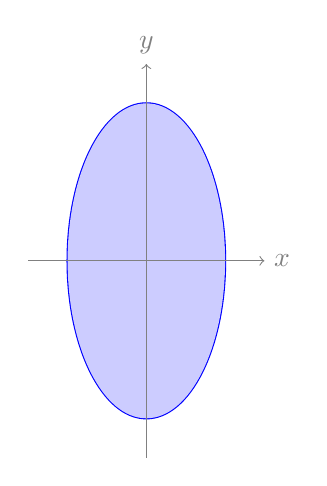
\begin{tikzpicture}[scale=1]
    \draw[thick, blue] (0,0) ellipse (1 and 2);
    \fill[blue!20] (0,0) ellipse (1 and 2);
    \draw[->, gray] (-1.5,0) -- (1.5,0) node[right] {$x$};
    \draw[->, gray] (0,-2.5) -- (0,2.5) node[above] {$y$};
    \end{tikzpicture}
    \end{center}
    令$\frac{\partial z}{\partial x} =\frac{\partial z}{\partial y} = 0$ 即$\begin{cases}
        2x = 0\\
        2y = 0
    \end{cases} \implies x = y = 0$ 故在内部仅有唯一驻点$(0,0)$,且$z\big|_{(0,0)}=2$ \\
    求条件极值 \\
    (方法一) 设拉格朗日函数为$\displaystyle L(x,y,\lambda)=x^2-y^2+2+\lambda(x^2+\frac{y^2}{4}-1)$ 分别对$x,y,\lambda$求导有
    \begin{align}
        L'_x=2x+2x\lambda = 0\tag{1} \\
        L'_y=2y+2y\lambda = 0\tag{2} \\
        L'_\lambda = x^2+\frac{y^2}{4} - 1 = 0 
    \end{align}
    此时有
    $$
    \begin{cases}
        x = 0, & y =\pm 2, f(0, \pm 2) = -2 \\
        y = 0, & x = \pm 1 f(\pm 1, 0) = 3 
    \end{cases}
    $$
    而当$x\neq 0\text{或}y\neq 0$时候与题设矛盾, 综上可知闭区间最值为
    $$
    \begin{cases}
        \text{最小值} d\big|_{0,\pm 2} = -2 \\
        \text{最大值} d\big|_{\pm 1, 0} = 3
    \end{cases}
    $$
    (方法二)有题设可知$y^2=4(1-x^2)$ 带入$f(x,y)\implies f(x)=x^2-4(1-x^2)+2 = 
    5x^2 - 2,x\in\left[-1,1\right]$ 显然当$x=0,f_{min}(x)=-2;x=\pm 1,f(x)=3$ \\
    (方法三) 令
    $
    \begin{cases}
        x = \cos{\theta} \\
        y = 2\sin{\theta}
    \end{cases}
    $ 其中$\theta\in\left[0,2\pi\right]$,此时$f(\theta)=\cos^2{\theta}-4\sin^2{\theta}+2=3-5\cos^2{\theta}$
    容易得出$f_{max}= 3;f_{min}=-2$
\end{solution} 
\end{enumerate}

\ifx\allfiles\undefined
\end{document}
\fi